\documentclass{standalone}

\usepackage{tikz}
\usetikzlibrary{shapes}

\newcommand{\Enc}{\ensuremath{\mathsf{Enc}}}
\newcommand{\Mac}{\ensuremath{\mathsf{Tag}}}

\begin{document}

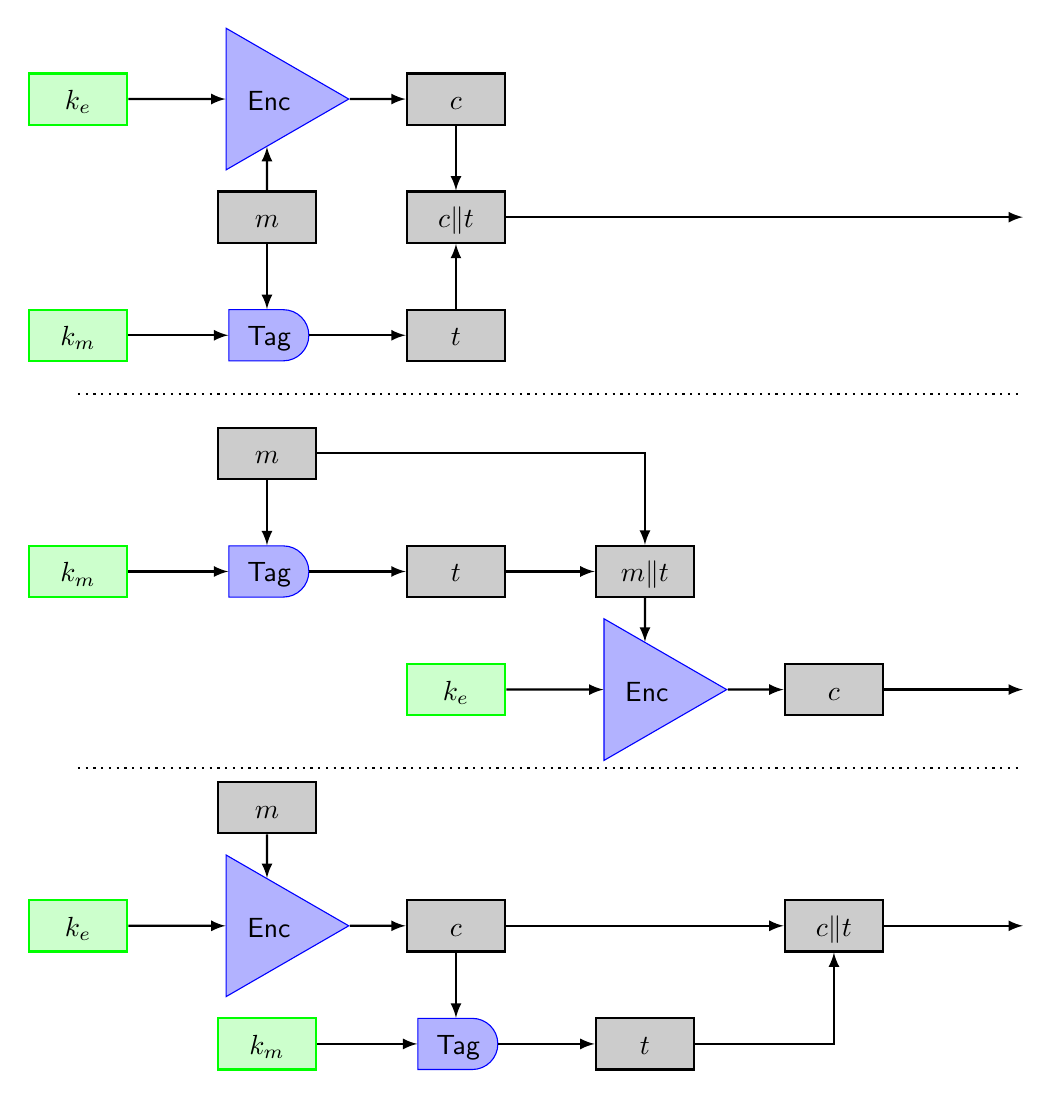
\begin{tikzpicture}[yscale=-1,xscale=0.8,>=latex]
				\tikzstyle{keys} = [thick, minimum width=1.25cm, minimum height=0.65cm, text height=2ex, text depth=0.25ex]
				\tikzstyle{key} = [keys, draw=green, fill=green!20]
				\tikzstyle{msg} = [keys, draw=black, fill=black!20]
				\tikzstyle{ctxt} = [keys, draw=black, fill=black!20]
				\tikzstyle{tag} = [keys, draw=black, fill=black!20]
				\tikzstyle{RECTRO} = [rounded rectangle, rounded rectangle west arc=0pt, minimum width=1.25cm, minimum height=0.65cm, text height=2ex, text depth=0.25ex]
				\tikzstyle{RORECT} = [rounded rectangle, rounded rectangle west arc=0pt, minimum width=1.25cm, minimum height=0.65cm, text height=2ex, text depth=0.25ex]
				\tikzstyle{SQUA} = [thick, minimum width=1.25cm, minimum height =1.25cm, text height=2ex, text depth=0.25ex]
				\tikzstyle{GEN} = [SQUA, draw=green, fill=green!20]
				\tikzset{triangle/.style={draw,	shape border rotate=180,regular polygon,regular polygon sides=3, minimum height=0.65cm}}
				\tikzstyle{ENC} = [triangle, text width=0.5cm, shape border rotate=270, text height=2ex, draw=blue, fill=blue!30]
				\tikzstyle{DEC} = [triangle, text width=0.5cm, shape border rotate=90, text height=2ex, draw=red, fill=red!30]
				\tikzstyle{MAC} = [RECTRO, text width=0.5cm, shape border rotate=90, text height=2ex, draw=blue, fill=blue!30]
				
				\node[key] (EncKey) at 	(0,0) {$k_e$};
				\node[key] (MacKey) at 	(0,3) {$k_m$};
				\node[msg] (ptxt) at   	(3,1.5) {$m$};
				\node[ENC] (Enc) at (3,0) {$\Enc$};
				\node[MAC] (Mac) at (3,3) {$\Mac$};
				\node[ctxt] (ctxt) at (6,0) {$c$};
				\node[tag] (tag) at (6,3) {$t$};
				\node[ctxt] (final) at (6,1.5) {$c\|t$};
				\draw[->, thick] (EncKey.east) -- (Enc.west);
				\draw[->, thick] (ptxt.north) -- (Enc.south);
				\draw[->, thick] (ptxt.south) -- (Mac.north);
				\draw[->, thick] (Enc.east) -- (ctxt.west);
				\draw[->, thick] (MacKey.east) -- (Mac.west);
				\draw[->, thick] (Mac.east) -- (tag.west);
				\draw[->, thick] (final.east) -- (15,1.5);
				\draw[->, thick] (tag.north) -- (final.south);
				\draw[->, thick] (ctxt.south) -- (final.north);
				
				\node[key] (MacKeyTwo) at 	(0,6) {$k_m$};
				\node[msg] (PtxtTwo) at (3,4.5) {$m$};
				\node[MAC] (MacTwo) at (3,6) {$\Mac$};
				\node[tag] (TagTwo) at (6,6) {$t$};
				\node[msg] (Concat) at (9,6) {$m \| t$};
				\node[key] (EncKeyTwo) at (6,7.5) {$k_e$};
				\node[ENC] (EncTwo) at (9,7.5) {$\Enc$};
				\node[ctxt] (CtxtTwo) at (12,7.5) {$c$};
				\draw[->, thick] (MacKeyTwo.east) -- (MacTwo.west);
				\draw[->, thick] (PtxtTwo.south) -- (MacTwo.north);
				\draw[->, thick] (MacTwo.east) -- (TagTwo.west);
				\draw[->, thick] (PtxtTwo.east) -| (Concat.north);
				\draw[->, thick] (TagTwo.east) -- (Concat.west);
				\draw[->, thick] (Concat.south) -- (EncTwo.north);
				\draw[->, thick] (EncKeyTwo.east) -- (EncTwo.west);
				\draw[->, thick] (EncTwo.east) -- (CtxtTwo.west);
				\draw[->, thick] (CtxtTwo.east) -- (15,7.5);
				
				\node[key] 	(EncKeyThree) at 	(0,10.5) 	{$k_e$};
				\node[msg] 	(PtxtThree) at 		(3,9) 		{$m$};
				\node[ENC] 	(EncThree) at 		(3,10.5) 	{$\Enc$};
				\node[ctxt] (CtxtThree) at 		(6,10.5) 	{$c$};
				\node[msg] 	(ConcatTwo) at 		(12,10.5) 	{$c \| t$};
				\node[key] 	(MacKeyThree) at 	(3,12) 		{$k_m$};
				\node[MAC] 	(MacThree) at 		(6,12) 		{$\Mac$};
				\node[ctxt] (TagThree) at 		(9,12) 		{$t$};
				\draw[->, thick] (EncKeyThree.east) -- (EncThree.west);
				\draw[->, thick] (PtxtThree.south) -- (EncThree.north);
				\draw[->, thick] (EncThree.east) -- (CtxtThree.west);
				\draw[->, thick] (CtxtThree.east) -- (ConcatTwo.west);
				\draw[->, thick] (CtxtThree.south) -- (MacThree.north);
				\draw[->, thick] (TagThree.east) -| (ConcatTwo.south);
				\draw[->, thick] (MacKeyThree.east) -- (MacThree.west);
				\draw[->, thick] (MacThree.east) -- (TagThree.west);
				\draw[->, thick] (ConcatTwo.east) -- (15,10.5);
				
				\draw[-,thick,dotted] (0,3.75) -- (15,3.75); 
				\draw[-,thick,dotted] (0,8.5) -- (15,8.5); 
				
\end{tikzpicture} 
\end{document}
